\section{Intro}

Neural networks became increasingly popular as showed by the \href{https://www.kdnuggets.com/2021/05/winning-machine-learning-competition.html}{research publication topics} of the recent years. The main advantage of those models is that they can learn complex structures and are highly customizable. However, one significant drawback is their poor explanability power. Neural networks are often categorized in the so-called "black box models" that are hard to understand.
Fortunately, there are some very good tutorials on understanding how a neural network actually works. The tutorials of \href{https://www.coursera.org/learn/neural-networks-deep-learning}{Andrew Ng} is an example of some very good materials available online. \\

I personally find out that a 1-layer network is relatively easy to understand, however it gets tricky when increasing the number of layers. This article is an attempt to understand in details the 2-layer neural network through the building of a small playground. We will even publish the playground online! To enjoy fully this article, the reader must be familiar with the working of a 1-layer neural network.\\

The difference between a 1-layer network and a 2-layer network relies in the following picture: \\

\begin{center}
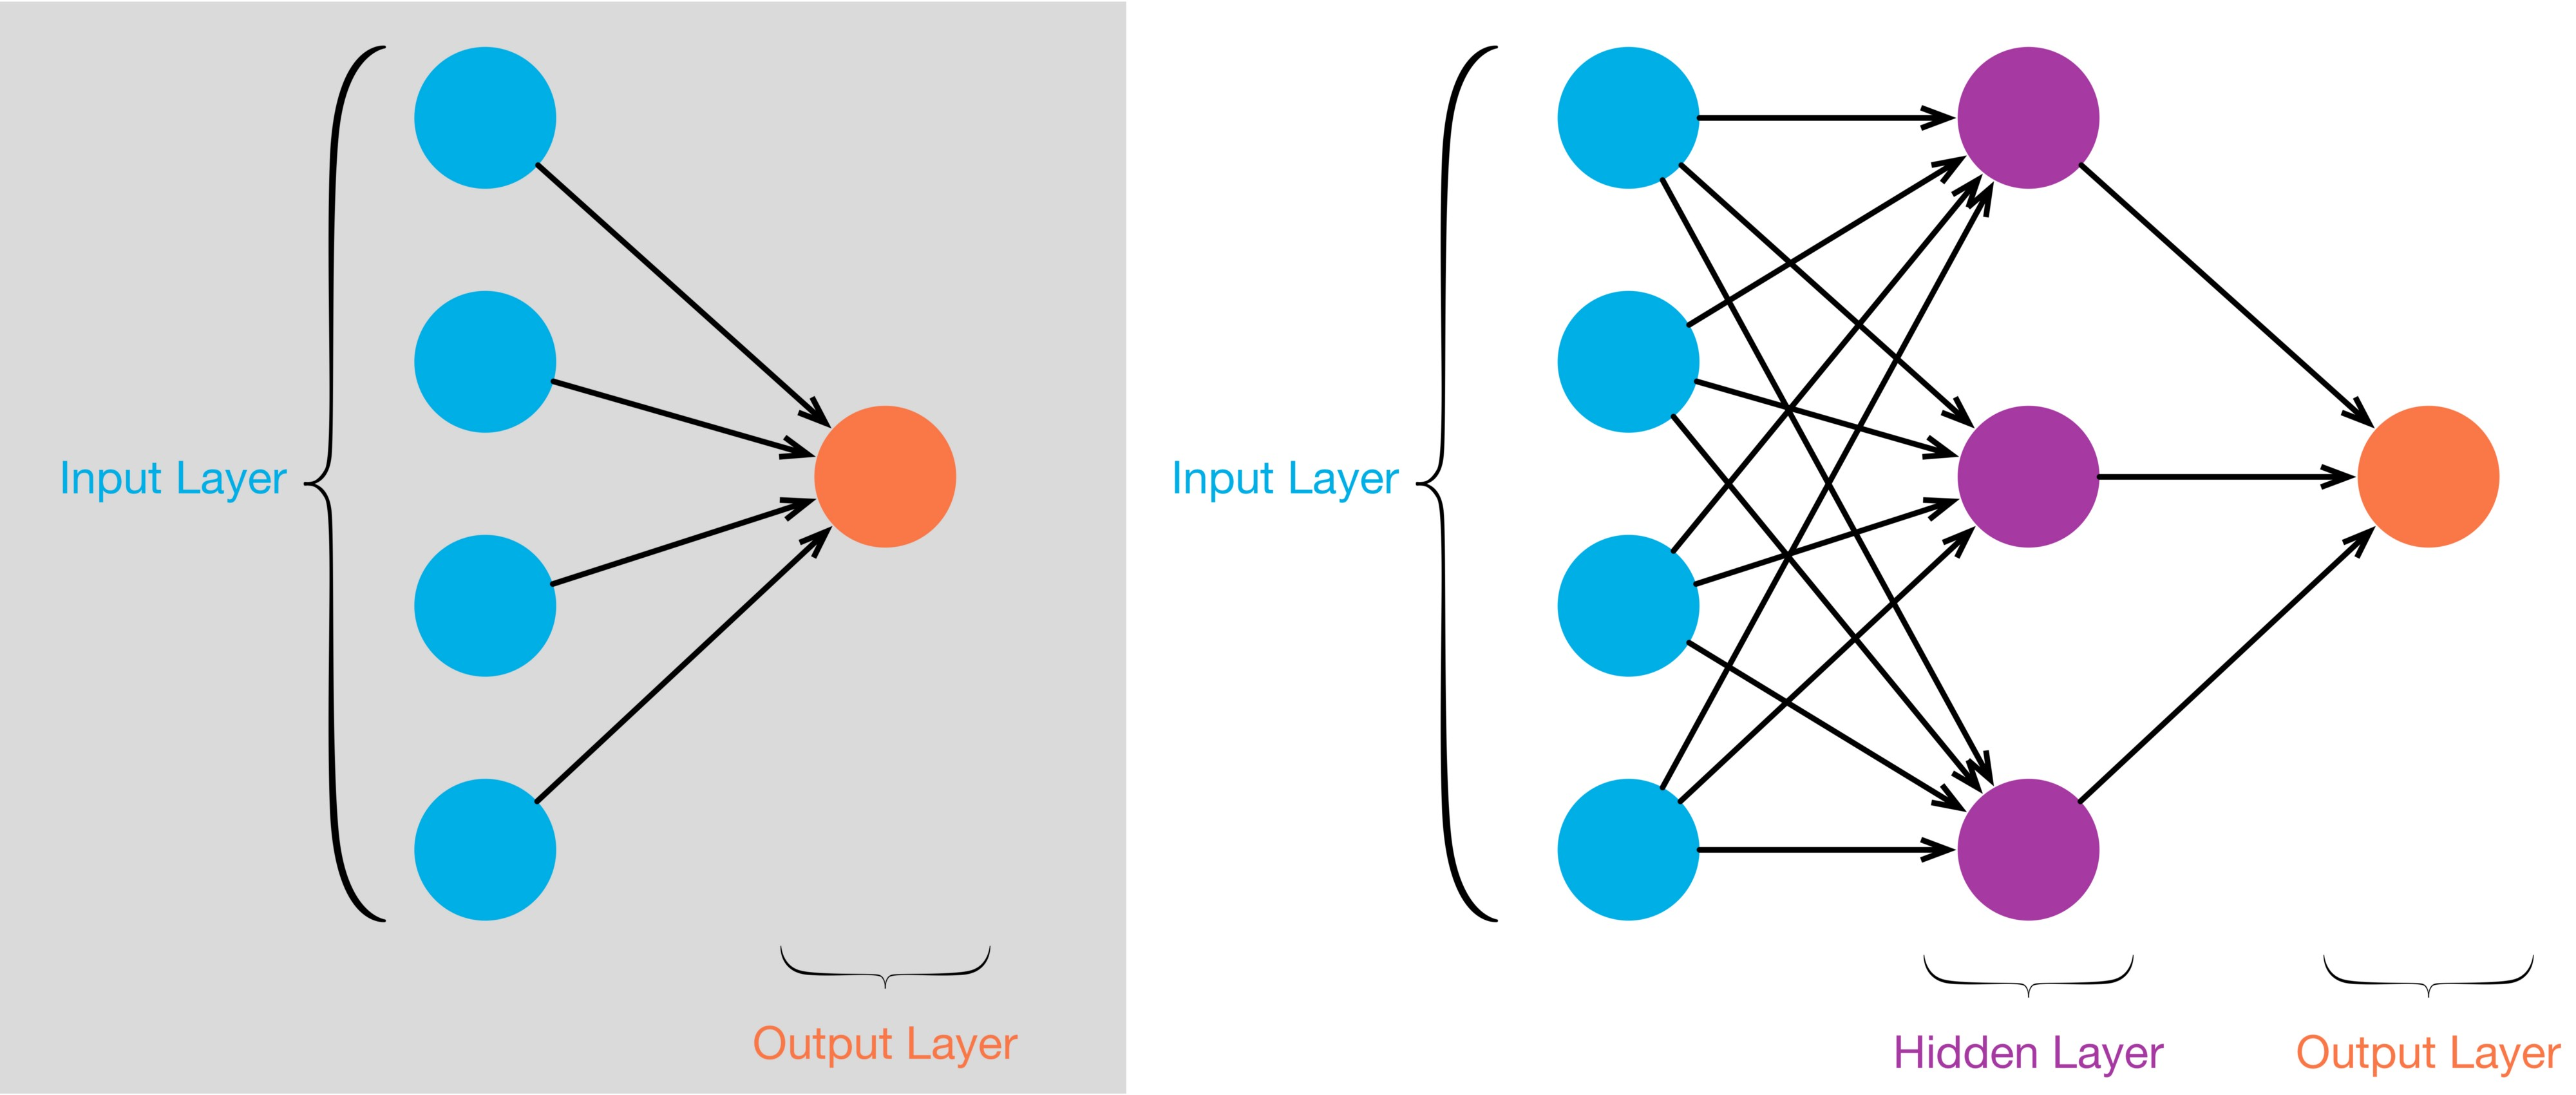
\includegraphics[scale=0.09]{img/nn-layers.jpeg}
\end{center}

Note that the input layer is usually ignored when counting the layers. \\

To understand deeply the 1-layer I strongly recommend Andrew Ng's tutorial for more details or this \href{https://towardsdatascience.com/everything-you-need-to-know-about-neural-networks-and-backpropagation-machine-learning-made-easy-e5285bc2be3a}{article} for a wrap up. \\

Let's now go into deeper details on the working on a 2-layer network.
